\documentclass[dvisvgm,border=8pt]{standalone}
\usepackage{amsmath,amssymb}
\usepackage[scaled]{helvet}\renewcommand{\familydefault}{\sfdefault}
\usepackage{tikz}\usetikzlibrary{positioning,arrows.meta,calc}
\definecolor{gin}{HTML}{F5F5F5}\definecolor{gstroke}{HTML}{666666}
\definecolor{dg}{HTML}{6D8764}\definecolor{dgs}{HTML}{3A5431}
\definecolor{exg}{HTML}{2E7D32}\definecolor{warn}{HTML}{B46504}
\newcommand{\ex}[1]{\textcolor{exg}{#1}}
\tikzset{font=\small, >={Stealth[length=2.2mm]},
  base/.style={draw, rounded corners=3pt, align=center, inner sep=5pt, minimum height=9mm},
  inp/.style={base, fill=gin, draw=gstroke},
  calc/.style={base, fill=white, draw=black},
  res/.style={base, fill=dg, draw=dgs, text=white},
  ar/.style={->, thick}}
\begin{document}
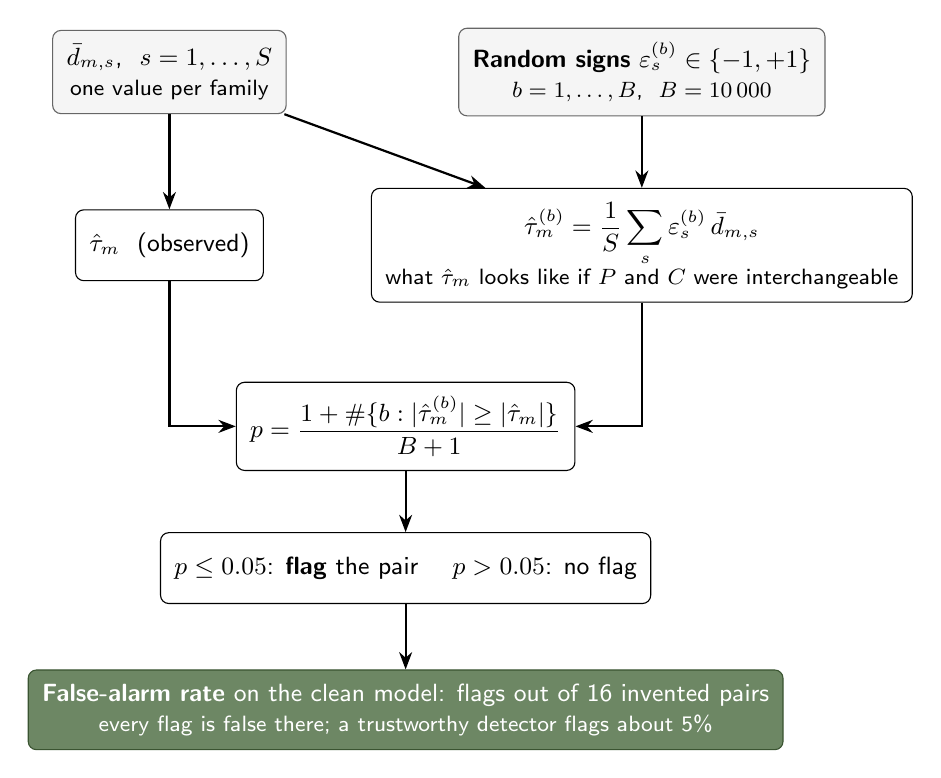
\begin{tikzpicture}
\node[inp] (D) at (0,0) {$\bar d_{m,s}$, \ $s=1,\dots,S$\\{\footnotesize one value per family}};
\node[inp] (E) at (6,0) {\textbf{Random signs} $\varepsilon^{(b)}_s\in\{-1,+1\}$\\{\footnotesize $b=1,\dots,B$, \ $B=10\,000$}};
\node[calc] (T) at (0,-2.2) {$\hat\tau_m$ \ (observed)};
\node[calc] (TB) at (6,-2.2) {$\hat\tau^{(b)}_m=\dfrac1S\displaystyle\sum_s\varepsilon^{(b)}_s\,\bar d_{m,s}$\\{\footnotesize what $\hat\tau_m$ looks like if $P$ and $C$ were interchangeable}};
\node[calc] (P) at (3,-4.5) {$p=\dfrac{1+\#\{b:|\hat\tau^{(b)}_m|\ge|\hat\tau_m|\}}{B+1}$};
\node[calc] (R) at (3,-6.3) {$p\le 0.05$: \textbf{flag} the pair \quad $p>0.05$: no flag};
\node[res] (F) at (3,-8.1) {\textbf{False-alarm rate} on the clean model: flags out of 16 invented pairs\\{\footnotesize every flag is false there; a trustworthy detector flags about 5\%}};
\draw[ar] (D) -- (T); \draw[ar] (D) -- (TB); \draw[ar] (E) -- (TB);
\draw[ar] (T) |- (P); \draw[ar] (TB) |- (P); \draw[ar] (P) -- (R); \draw[ar] (R) -- (F);
\end{tikzpicture}
\end{document}
